%!TEX root = ../main.tex

\subsection{Normal component}\label{ss:normal_component}
% What?
In this section we discuss the parametrization of the normals. How the computed normals are actually a kind of `fake' normals. The real normals being the normals that are calculated using the geometry of the PN triangle thus a cubic B\`ezier surface. Section \ref{sss:method:normals:fakeNormals} and \ref{sss:method:normals:realNormals} provide the formulas and explanation for both types of normals and their construction. 

Additionally as with the geometry of the PN triangle we again only have the information from the input primitive available i.e. the vertices positions and normals (see figure \ref{fig:method:input_primitive}).

\begin{figure}
	\centering
	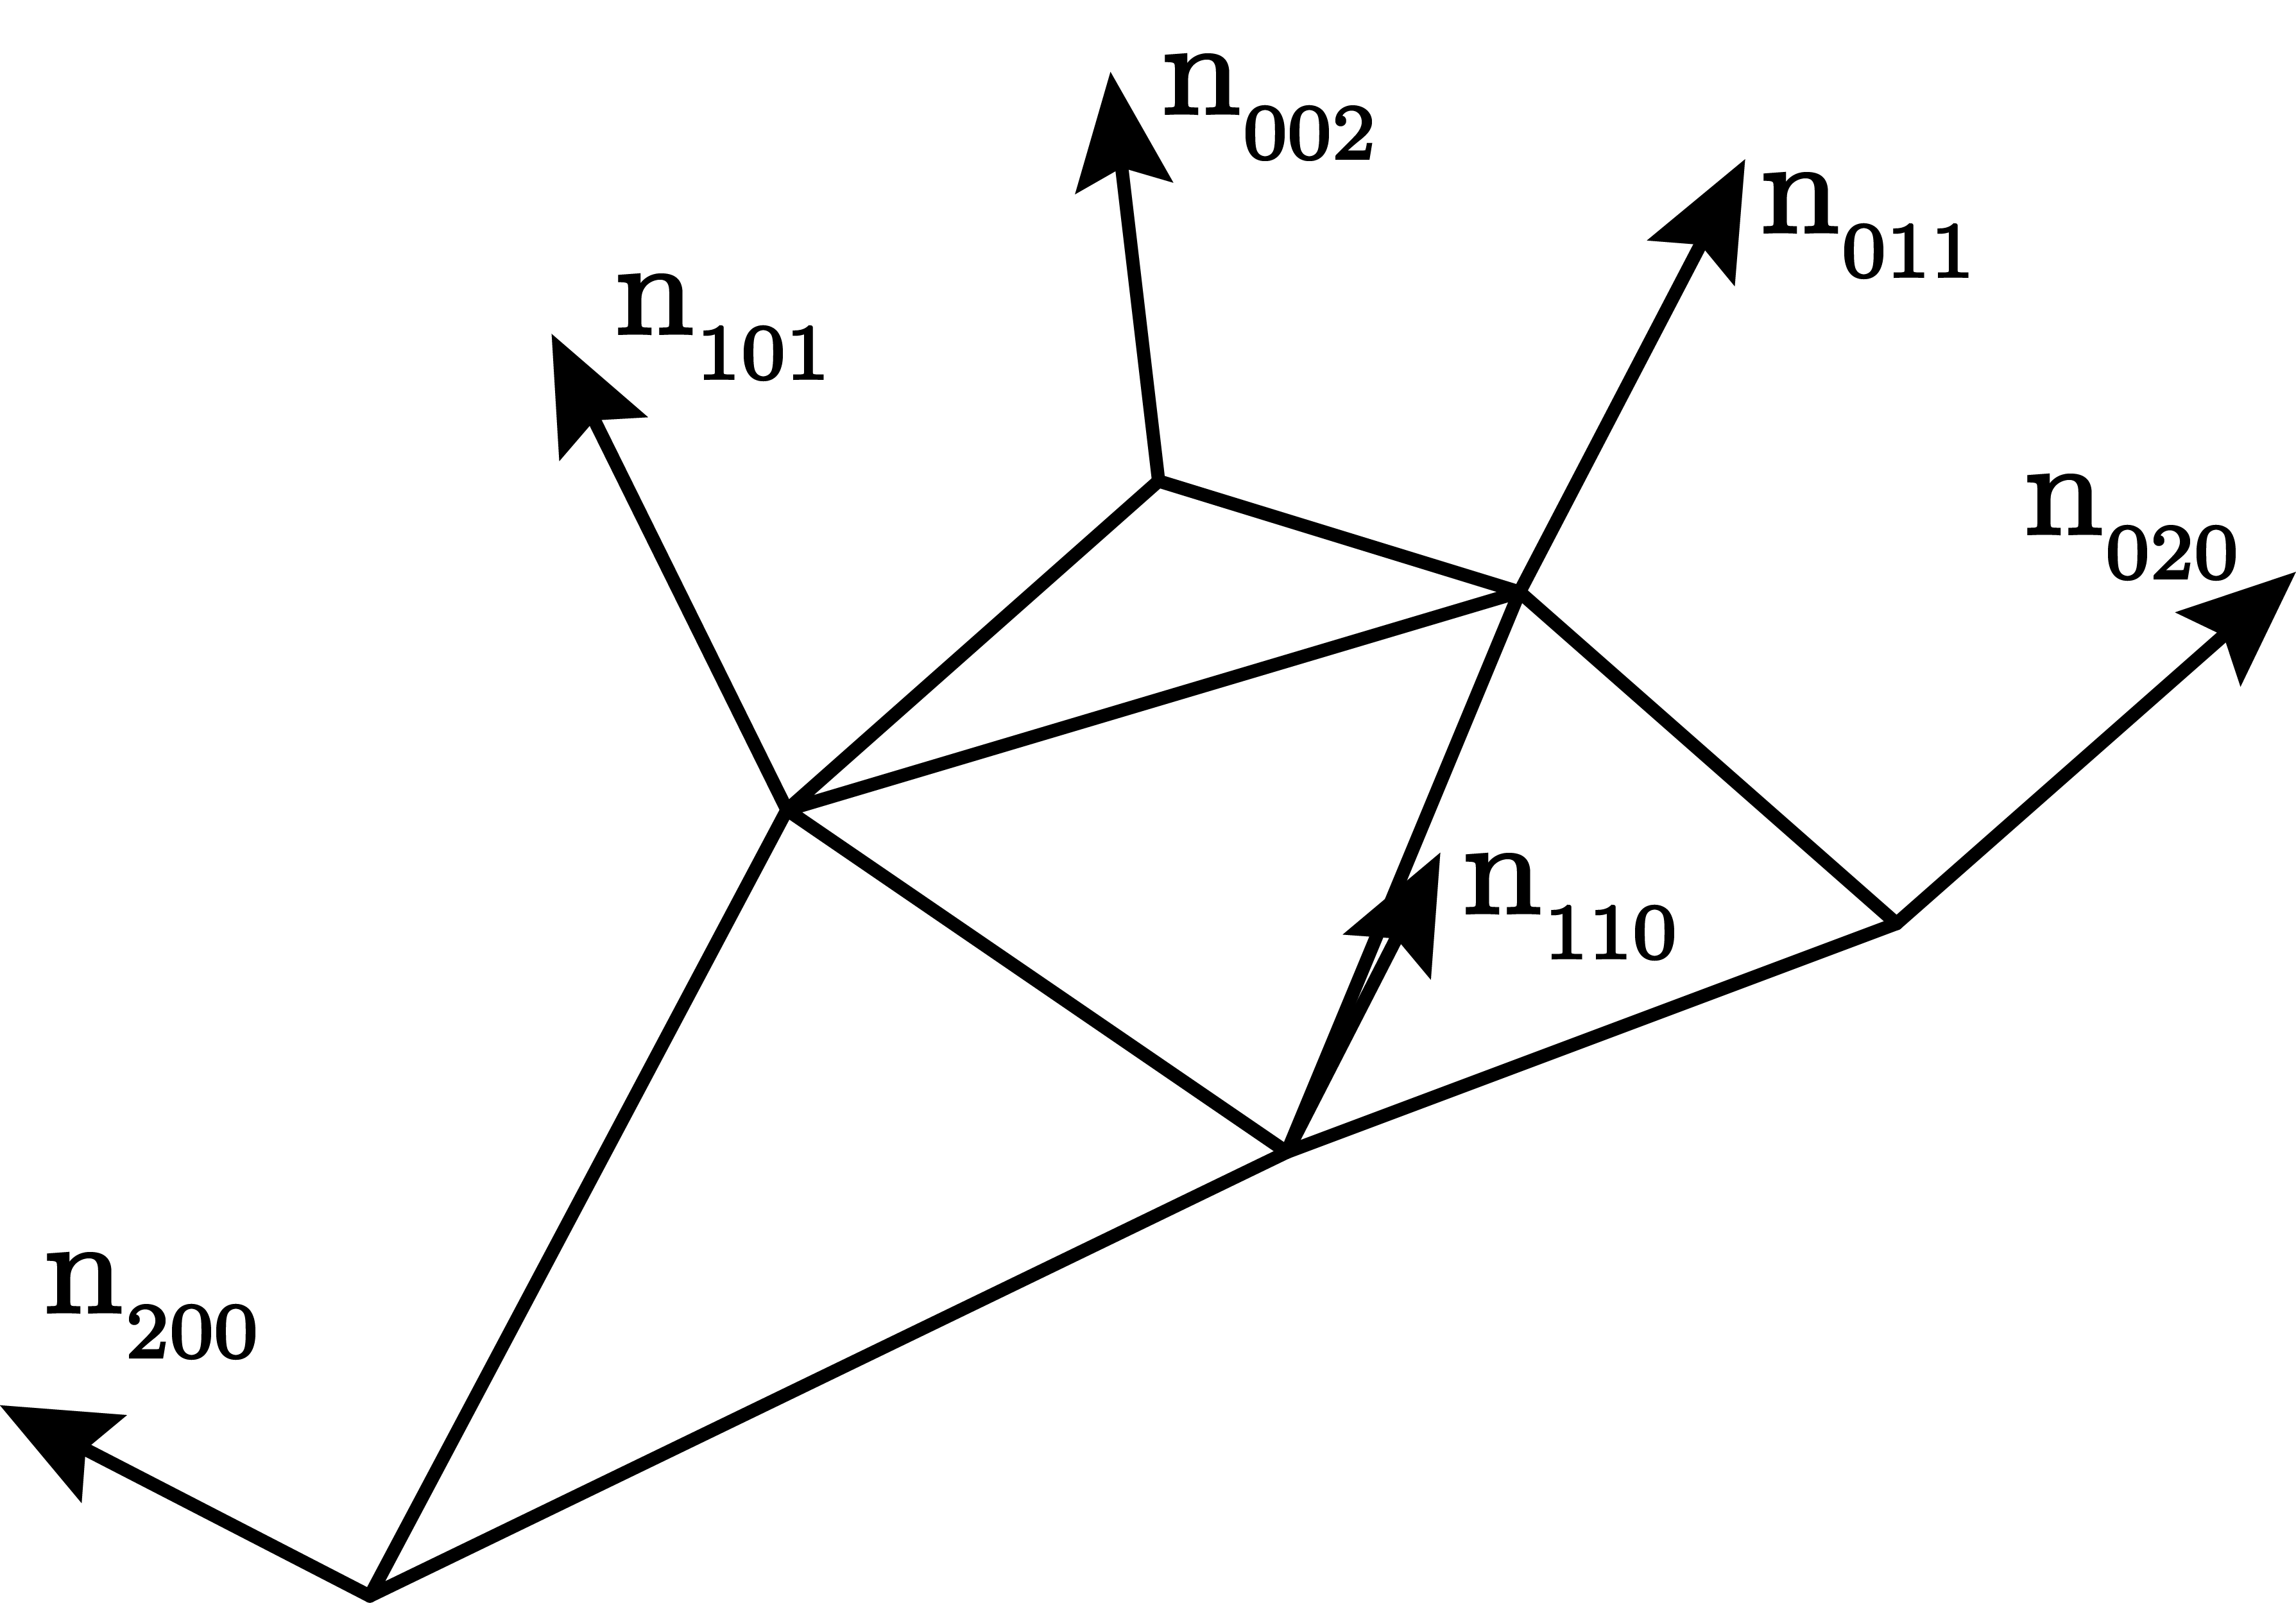
\includegraphics[width=0.45\textwidth]{./content/img/method/normals.png}
	\caption{The normal field of the PN triangle}
	\label{fig:method:normal_field}
\end{figure}

\subsubsection{Fake normals}\label{sss:method:normals:fakeNormals}
The `fake' normals following the definition from \citeauthor{vlachos2001curved} and are defined by the the quadratic function $n$: 
\begin{align}
\noalign{$n: \quad R^2 \mapsto R^3,\quad$ for $w = 1 - u - v, \quad u, v, w \geq 0$}
\begin{split}\label{eq:method:quadratic_normal_patch}
    n(u,v) ={}& \sum_{i + j + k = 2} n_{ijk}u^i v^j w^k,\\
      	   ={}& n_{200}w^2 + n_{020}u^2 + n_{002}v^2\\
      	    {}& + n_{110}wu + n_{011}uv + n_{101}wv\\
\end{split}
\end{align}
The coefficients of this quadratic `patch' are the normals shown in figure \ref{fig:method:normal_field}. The normals are computed for the point, halfway every edge. The reason why quadratically varying normals are used is, to capture the inflection points that are possible because of the use of the cubic patch for the geometry of the triangle. Figure \ref{fig:method:linear_vs_quadratically_varying} illustrates two cases: the top two images show a parabolic curve where both linear and quadratically varying normals perform the same. The more interesting case is the one illustrated by the two bottom images that show a cubic curve. We see that the linear varying normals do not capture the correct normal for this curve, but the quadratic varying normals do.

\begin{figure}
	\centering
	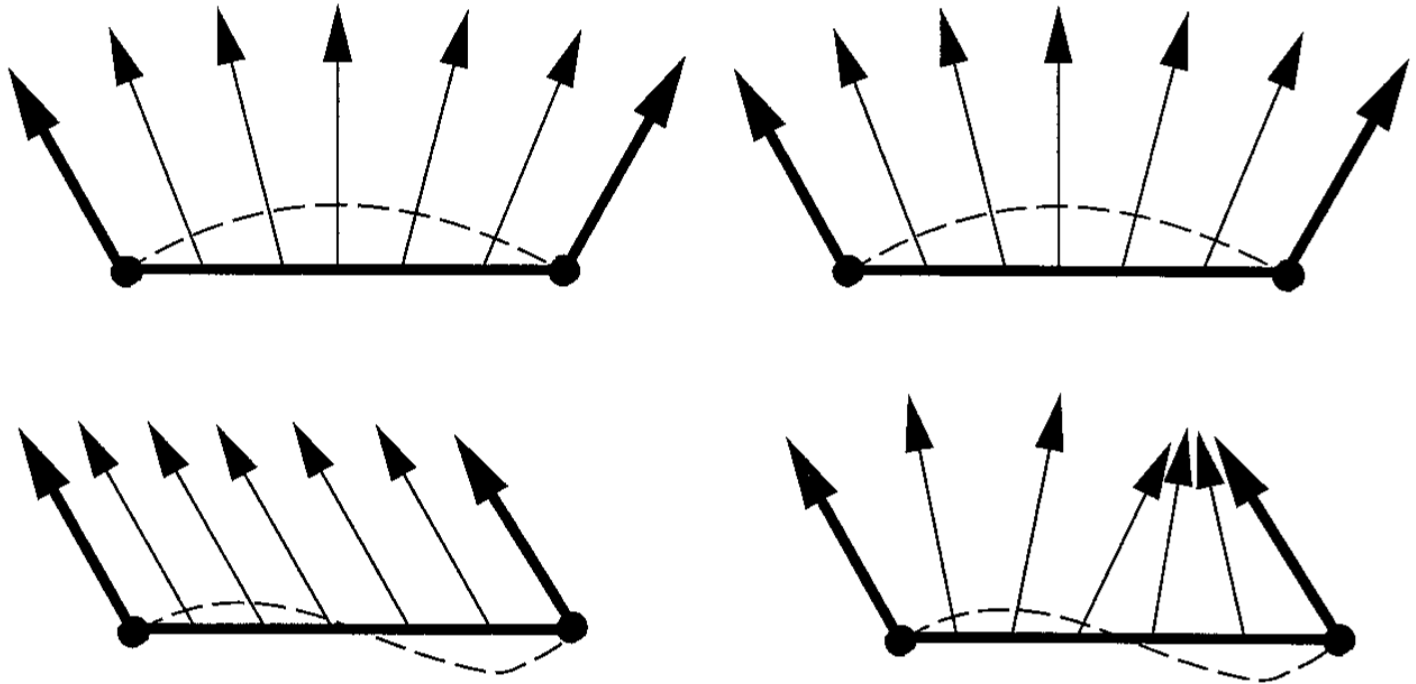
\includegraphics[width=0.45\textwidth]{./content/img/method/lin_vs_quad_varying_normals(inspiration).png}
	\caption{\textit{left:} linear varying normals. \textit{right:} quadratically varying normals. Taken from \citeauthor{van1997phong}}
	\label{fig:method:linear_vs_quadratically_varying}
\end{figure}
\todo[inline]{Discuss parametrization of `quadratic' patch}

Using the function $n$ the normal of any point parametrized by the barycentric coordinates $u, v$ can be calculated. To be able to do this the control points first need to be constructed. We group the coefficient into two groups: the vertex normals, $n_{200}$, $n_{020}$, and $n_{002}$; and the edge normals, $n_{110}$, $n_{011}$, and $n_{101}$. \todo{and some more text.}
\todo[inline]{Discuss the construction of the control points for the `quadratic' patch}

\subsubsection{Real normals}
\label{sss:method:normals:realNormals}
	\todo[inline]{Discuss how to compute the real normals given the geometric component}
	The real normals are computed using the points on the cubic B\`ezier patch. This can be done by taking the cross product of the the partial derivative with respect to $u$ and $v$.
